\documentclass[a4paper]{article}
\usepackage[dutch]{babel}
\usepackage[utf8x]{inputenc}
\usepackage{amsmath,graphicx,hyperref,parskip,setspace,fancyhdr,changepage}
\usepackage[margin=1in]{geometry}
\usepackage[colorinlistoftodos]{todonotes}

\setlength{\parindent}{0mm}
\linespread{1.4}

\newcommand{\rcom}[1]{\textbf{\textcolor{red}{#1}}}
\newcommand{\com}[2]{\texttt{#1}\mbox{}\vspace{-2ex}\begin{adjustwidth}{0.8cm}{} #2 \end{adjustwidth}}

\pagestyle{fancy}

\title{Symbolische manipulatie}
\author{Rik~Voorhaar~(3888169) - Jan-Willem~van~Ittersum~(3992942) - Jurre~Corver~(3905985)\\
Begeleider: Joost Houben}

\begin{document}
\maketitle
\clearpage

%\begin{abstract}
%Your abstract.
%\end{abstract}

\rcom{Gisteren met Joost gesproken over het verslag. Hij zei dat alle standaardfuncties best op een regel in de documentatie mogen. Bovendien vond hij het niet erg als het verslag iets langer dan 5 pagina's is (zolang er maar nuttige dingen in staan). }

\section{Introductie}
In deze opdracht hebben we een eigen computeralgebrasysteem (CAS) ontwikkeld om symbolisch te kunnen rekenen zoals dat bijvoorbeeld in Mathematica gebeurt. Wiskundige formules worden hiervoor opgeslagen in een zogenaamde expressie-boom. Behalve dat deze representatie kan worden gebruikt om berekeningen te doen, is deze geschikt voor symbolische manipulaties, zoals optellen, vermenigvuldigen, maar ook differenti\"eren en oplossen van sommige polynoom~vergelijkingen. De code behordende bij dit project kan gevonden worden op \url{https://github.com/JurreCorver/SymbolischeManipulatie}.


\section{Theorie}
%Beschrijving van de theorie
Een expressie-boom is een samenhangende, gerichte graaf, waarbij elke knoop (op \'e\'en knoop na) exact \'e\'en inkomende zijde heeft en een willekeurig aantal uitgaande zijden. De unieke knoop zonder inkomende zijde noemen we \textit{de wortel}, een knoop met minstens \'e\'en uitgaande zijde noemen we \textit{een interne knoop} en een knoop zonder uitgaande zijde noemen we \textit{een blad}. In de knopen van deze expressie-boom wordt een berekening opgeslagen. Een blad is een constante of een variabele, bijvoorbeeld $3$ of $x$. Een interne knoop (de wortel is ook een interne knoop) is een operator of een functie. Naast de binaire operatoren optellen $+$, aftrekken $-$, vermenigvuldigen $*$, delen $/$, modulo $\%$ en machtsverheffing $**$ die gekenmerkt worden door het feit dat er zowel links als rechts van de operator \'e\'en argument nodig is, is er een negatie operator $-$ die alleen een argument rechts heeft. Vergelijk bijvoorbeeld de binaire operator $-$ in $5-x$ met de negatie operator $-$ in $-x+2$. Een voorbeeld van een expressieboom zie je in \rcom{Ik weet niet hoe je handig plaatjes kan maken, maar ik stel voor om de expressie $-2+\sin(1.2*3)$ o.i.d. in een expressieboom te zetten (in ieder geval minstens \'e\'en functie,  \'e\'en negNode en  \'e\'en binaire knoop}. 


\section{Algoritmen}
%Beschrijving van de gebruikte algoritmen, denk hierbij ook aan bijvoorbeeld de complexiteit en de gebruikte datastructuren
\subsection{Shunting-Yard}


\section{Documentatie}
%Documentatie over het gebruik van de code
\subsection{Installatie}
Om dit programma te gebruiken zijn naast een werkende Python 3.4 distributie enkele Python packages nodig. De niet-standaard packages zijn: \texttt{numpy, pillow, scipy, tkinter}.
Verder heeft de grafische gebruikers omgeving onderstuining voor het weergeven van de output met behulp van \LaTeX. Hiervoor is dus een werkende \LaTeX~distributie vereist. Daarbij is het ook benodigd om \emph{GhostScript} geinstalleerd te hebben. Voor \emph{Windows} gebruikers is het verder specifiek vereist om de 32-bit versie van \emph{GhostScript} te gebruiken en het pad naar \texttt{gswin32c.exe} toe te voegen aan de \texttt{\%path\%} systeemvariabele.

\subsection{Grafische omgeving}
De grafische omgeving kan gebruikt worden door \texttt{tkmain.pyw} uit te voeren. Dit kan ook vanuit de command-line door \texttt{python tkmain.pyw} uit te voeren.  De verschillende componenten van de omgeving zullen worden uitgelegd met referentie naar figuur \ref{fig:screenshot}

\begin{figure}[!htb]
  \centering
  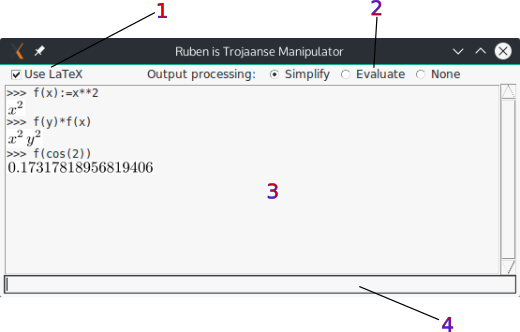
\includegraphics[width=0.6\textwidth]{screenshot.png}
  \caption{Screenshot van de grafische omgeving}
  \label{fig:screenshot}
\end{figure}

\begin{enumerate}
\item Met de \texttt{Use LaTeX} wordt gespecificeerd of de output door \LaTeX wordt verwerkt voor dat deze wordt weergegeven. Indien deze optie niet geselecteerd is zal de output als plain-text worden weergegeven.
\item De \texttt{Output processing} optie specificeerd hoe de input wordt verwerkt. Indien \texttt{Simplify} is aangevinkt zal de expressie zo veel mogelijk versimpeld worden. Terwijl bij het aanvinken van \texttt{Evaluate} de expressie wordt uitgerekend indien deze numeriek is, en anders onversimpeld wordt weergegeven. Als laatste zorgt de \texttt{None} optie juist dat de expressie niet wordt berekend en direct wordt weergegeven.
\item Dit is het scherm waar de output wordt weergegeven. Hier wordt de input van de gebruiker met \texttt{>>>} er voor weergegeven, en telkens op de regel daarna de output bij de regel input erboven. Indien er fouten optraden tijdens het uitvoeren van de input wordt dit hier ook weergegeven.
\item In dit scherm kan de gebruiker zijn input invoeren. Als de gebruiker de \texttt{Enter} toets indrukt wordt de input ge\"evaluaeerd. De pijltjestoetsen naar boven en onder kunnen worden gebruikt om de vorige input nog een keer te gebruiken.
\end{enumerate}

\subsection{Syntax}
De invoer ondersteund standaard operaties op getallen die met symbolen \texttt{*, +, -, **, /, \%} kunnen worden ingevoerd. Verder kunnen ronde haaken \texttt{( )} worden gebruikt. Enkele voorbeelden:
\begin{adjustwidth}{1.5cm}{}
\setstretch{0.9}
\texttt{>>> 2+2-1}\\
$1$\\
\texttt{>>> (2**3)/2}\\
$4$\\
\texttt{>>> 7 \% 3}\\
$1$
\end{adjustwidth}
Ook zijn standaard functies als \texttt{sin, ln, gamma, gcd} ge\"implementeerd. %De specifieke details over deze functies zijn te vinden in de volgende sectie. 
De lijst met alle ge\"implementeerde functies is te vinden in de volgende sectie. Er is verder ook ondersteuning voor complexe getallen. De imaginaire constante wordt aangeduid met \texttt{i}. Andere standaard constanten zijn \texttt{pi, e, phi}. Voorbeeld:
\begin{adjustwidth}{1.5cm}{}
\setstretch{0.9}
\texttt{>>> i**2}\\
$-1$\\
\texttt{>>> exp(i*pi)-1}\\
$0$\\
\end{adjustwidth}
Naast standaard operaties is het ook mogelijk om zelf functies en constanten toe te voegen. Hiervoor kan \texttt{:=} gebruikt worden. Als links van de \texttt{:=} alleen een symbool staat, dan wordt wat rechts van de \texttt{:=} staat opgeslagen onder naam van het symbool aan de linkerkant. We kunnen bijvoorbeeld het volgende doen:
\begin{adjustwidth}{1.5cm}{}
\setstretch{0.9}
\texttt{>>> x:=5}\\
$5$\\
\texttt{>>> x**2}\\
$25$
\end{adjustwidth}
Functies kunnen op een vergelijkbare manier worden toegevoegd. Neem als voorbeeld:
\begin{adjustwidth}{1.5cm}{}
\setstretch{1}
\texttt{>>> f(x,y):=sin(x)*cos(y)}\\
$\mathrm{sin}(x)\,\mathrm{cos}(y)$\\
\texttt{>>> f(pi/2,pi)}\\
$-1$
\end{adjustwidth}
Als laatste is er ondersteuning voor een gelijkheids operator met \texttt{==} als symbool. Deze kan bijvoorbeeld worden gebruikt bij invoeren van vergelijkingen.


\subsection{Lijst van commando's}
\rcom{na afloop op alfabetische volgorde zetten\\}
\com{exit()}{Sluit het programma af.}
\com{d(f(x),x)}{Berekent de afgeleide van \texttt{f(x)} naar de variabele \texttt{x}. Indien de afgeleide van de functie niet bekend is wordt een foutmelding gegeven. Voorbeeld:\vspace{-0.5ex}}
\begin{adjustwidth}{1.5cm}{}
\setstretch{1}
\texttt{>>> d(sin(x)+2,x)}\\
$\cos(x)$
\end{adjustwidth}

\com{sin(x), arcsin(x), cos(x), arccos(x), tan(x), arctan(x), ln(x), exp(x), floor(x), gamma(x)}{Geeft de bijbehorende standaardfunctie als functie van \texttt{x}.}
%\com{sin(x)}{Geeft de sinus van \texttt{x}.}
%\com{arcsin(x)}{Geeft de arcsinus van \texttt{x}.}
%\com{cos(x)}{Geeft de cosinus van \texttt{x}.}
%\com{arccos(x)}{Geeft de arccosinus van \texttt{x}.}
%\com{tan(x)}{Geeft de tangus van \texttt{x}.}
%\com{arctan(x)}{Geeft de arctangus van \texttt{x}.}
%\com{log(x,y)}{Geeft het logaritme van \texttt{x} in basis \texttt{y}. Equivalent aan \texttt{ln(x)/ln(y)}.}
%\com{ln(x)}{Geeft het natuurlijk logaritme van \texttt{x}.}
%\com{exp(x)}{Geeft het exponent van \texttt{x}.}
%\com{floor(x)}{Neemt de floor van \texttt{x}.}
%\com{gamma(x)}{Geeft de gamma functie van \texttt{x}.}
\com{log(x,y)}{Geeft het logaritme van \texttt{x} in basis \texttt{y}. Equivalent aan \texttt{ln(x)/ln(y)}.}
\com{polygamma(x,y)}{Geeft de \texttt{y}'de orde polygamma functie van \texttt{x}.}

\rcom{misschien ook nog even round en ceil toevoegen voor compleetheid?}

\rcom{nog toevoegen:\\}
\com{solvePolynomial(eq, var)}{}
\com{numIntegrate(expressie, x, l, r, numsteps)}{Numeriek bepalen van $\int_{\texttt{l}}^\texttt{r} \texttt{expressie} \; \mathrm{d}\texttt{x}$ door middel van een Riemann benadering in \texttt{numsteps} stappen.}
\com{gcd(n,m)}{Geeft de grootste gemene deler van twee gehele getallen \texttt{n} en \texttt{m}.}
\com{polQuotient(pol1, pol2, x)}{Geeft het quotient van de deling van \texttt{pol1} door \texttt{pol2} met rest, waarbij \texttt{pol1} en \texttt{pol2} polynomen in \texttt{x} zijn.}
\com{polRemainder(pol1, pol2, x)}{Geeft de rest van de deling van \texttt{pol1} door \texttt{pol2}, waarbij \texttt{pol1} en \texttt{pol2} polynomen in \texttt{x} zijn.}
\com{polIntQuotient(pol1, pol2, x)}{Geeft het quotient van de deling van het polynoom \texttt{pol1} door het polynoom \texttt{pol2} met rest over de gehele getallen, waarbij \texttt{pol1} en \texttt{pol2} polynomen met gehele co\"effici\"enten in \texttt{x} zijn.}
\com{polIntRemainder(pol1, pol2, x)}{Geeft de rest van de deling van \texttt{pol1} door \texttt{pol2} over de gehele getallen, waarbij \texttt{pol1} en \texttt{pol2} polynomen in \texttt{x} zijn.}
\com{polContent(pol,x)}{Geeft de content van het polynoom \texttt{pol} in \texttt{x}.}
\com{polGcd(pol1,pol2,x)}{Geeft de grootste gemene deler van twee polynomen \texttt{pol1} en \texttt{pol1} met gehele co\"effici\"enten in \texttt{x}.}
\com{deg(pol,x)}{Geeft de graad van \texttt{pol} als polynoom in \texttt{x}.}

\section{Resultaten}
%Eventuele resultate die behaald zijn met de code

\section{Taakverdeling}
%De taakverdeling binnen je groepje.





\begin{thebibliography}{99}

\bibitem{c1} Wikipedia - Shunting-yard algorithm:
\url{https://en.wikipedia.org/wiki/Shunting-yard_algorithm}. 
 - geraadpleegd op 28 juni 2015
 \bibitem{c2} Houben, Joost. Expressie-bomen en Symbolische Manipulatie: WISB256 – Programmeren in de Wiskunde.


\end{thebibliography}



\end{document}